\documentclass[tikz,border=8pt]{standalone}
\usepackage{amsmath}
\usetikzlibrary{arrows.meta}
\begin{document}
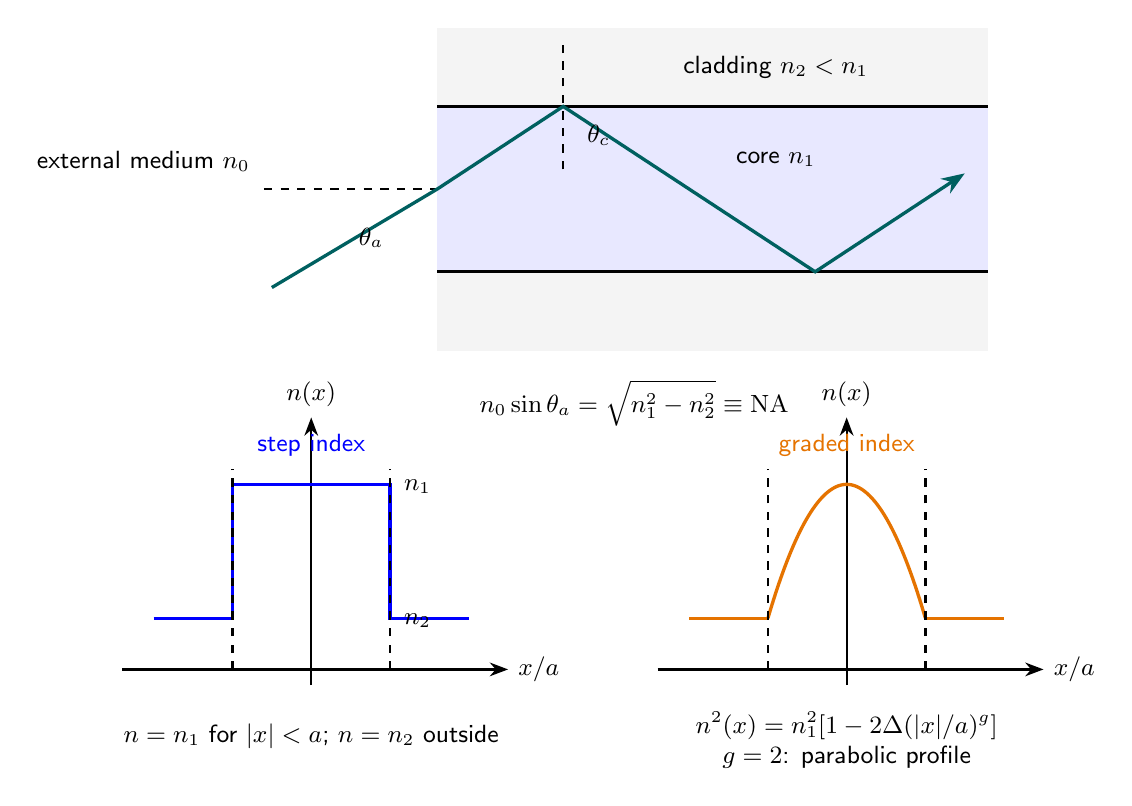
\begin{tikzpicture}[font=\sffamily\small,>=Stealth,thick]
  \begin{scope}[xshift=1.4cm]
    \fill[blue!9] (2,-1.05) rectangle (9,1.05);
    \fill[gray!9] (2,1.05) rectangle (9,2.05);
    \fill[gray!9] (2,-2.05) rectangle (9,-1.05);
    \draw[very thick] (2,1.05)--(9,1.05) (2,-1.05)--(9,-1.05);
    \draw[dashed] (-.2,0)--(2,0);
    \draw[->,teal!75!black,very thick] (-.1,-1.25)--(2,0)
      --(3.6,1.05)--(5.2,0)--(6.8,-1.05)--(8.7,.2);
    \draw[dashed] (3.6,.25)--(3.6,1.85);
    \node at (4.05,.68) {$\theta_c$};
    \node[anchor=east] at (1.45,-.62) {$\theta_a$};
    \node at (6.3,.38) {core $n_1$};
    \node at (6.3,1.55) {cladding $n_2<n_1$};
    \node[anchor=east] at (-.25,.35) {external medium $n_0$};
    \node[align=center] at (4.5,-2.72)
      {$\displaystyle n_0\sin\theta_a=\sqrt{n_1^2-n_2^2}\equiv\mathrm{NA}$};
  \end{scope}
  \begin{scope}[xshift=1.8cm,yshift=-6.1cm]
    \draw[->] (0,-.2)--(0,3.2) node[above] {$n(x)$};
    \draw[->] (-2.4,0)--(2.5,0) node[right] {$x/a$};
    \draw[blue,very thick] (-2,.65)--(-1,.65)--(-1,2.35)--(1,2.35)--(1,.65)--(2,.65);
    \draw[dashed] (-1,0)--(-1,2.55) (1,0)--(1,2.55);
    \node[blue] at (0,2.85) {step index};
    \node at (1.35,2.32) {$n_1$}; \node at (1.35,.62) {$n_2$};
    \node[align=center] at (0,-.85) {$n=n_1$ for $|x|<a$; $n=n_2$ outside};
  \end{scope}
  \begin{scope}[xshift=8.6cm,yshift=-6.1cm]
    \draw[->] (0,-.2)--(0,3.2) node[above] {$n(x)$};
    \draw[->] (-2.4,0)--(2.5,0) node[right] {$x/a$};
    \draw[orange!90!black,very thick,domain=-1:1,samples=100]
      plot (\x,{.65+1.70*(1-\x*\x)});
    \draw[orange!90!black,very thick] (-2,.65)--(-1,.65) (1,.65)--(2,.65);
    \draw[dashed] (-1,0)--(-1,2.55) (1,0)--(1,2.55);
    \node[orange!90!black] at (0,2.85) {graded index};
    \node[align=center] at (0,-.9)
      {$n^2(x)=n_1^2[1-2\Delta(|x|/a)^g]$\\$g=2$: parabolic profile};
  \end{scope}
\end{tikzpicture}
\end{document}
